\documentclass[%
    %handout
]{beamer}
\usepackage{cambridge_lecture}
\usepackage{hyperref}
\usepackage{graphicx}
\usepackage{amsmath}
\usepackage{calculator}

\newcommand{\cols}[3][0.5]{%
    \SUBTRACT{1.}{#1}{\wdthb}
    \begin{columns}
        \begin{column}{#1\textwidth}
            #2
        \end{column}
        \begin{column}{\wdthb\textwidth}
            #3
        \end{column}
    \end{columns}
}

\newcommand{\figname}{}
\newenvironment{figright}[2][0.5]{%
    \renewcommand{\figname}{#2}
    \SUBTRACT{1.}{#1}{\wdthb}
    \begin{columns}
        \begin{column}{#1\textwidth}
        }{%
        \end{column}
        \begin{column}{\wdthb\textwidth}
            \includegraphics[width=\textwidth]{\figname}
        \end{column}
    \end{columns}
}

\newcommand{\dfigname}{}
\newenvironment{dfigright}[3][0.5]{%
    \renewcommand{\figname}{#2}
    \renewcommand{\dfigname}{#3}
    \SUBTRACT{1.}{#1}{\wdthb}
    \begin{columns}
        \begin{column}{#1\textwidth}
        }{%
        \end{column}
        \begin{column}{\wdthb\textwidth}
            \includegraphics[width=\textwidth]{\figname}
            \includegraphics[width=\textwidth]{\dfigname}
        \end{column}
    \end{columns}
}



\newenvironment{figleft}[2][0.5]{%
    \SUBTRACT{1.}{#1}{\wdthb}
    \begin{columns}
        \begin{column}{#1\textwidth}
            \includegraphics[width=\textwidth]{#2}
        \end{column}
        \begin{column}{\wdthb\textwidth}
        }{%
        \end{column}
    \end{columns}
}

\newenvironment{dfigleft}[3][0.5]{%
    \SUBTRACT{1.}{#1}{\wdthb}
    \begin{columns}
        \begin{column}{#1\textwidth}
            \includegraphics[width=\textwidth]{#2}
            \includegraphics[width=\textwidth]{#3}
        \end{column}
        \begin{column}{\wdthb\textwidth}
        }{%
        \end{column}
    \end{columns}
}


\newcounter{numimages}

\newenvironment{multifig}[1]{%
    \begin{frame}
        \pdfximage{#1}%
        \setcounter{numimages}{\the\pdflastximagepages}
        \addtocounter{numimages}{-1}

        \begin{tikzpicture}[remember picture, overlay]
            \foreach \pagenum in {1,...,\thenumimages} {%
                \node<handout:0|beamer:\pagenum>[anchor=center] at (current page.center) {
                \includegraphics[width=\textwidth,page=\pagenum]{#1}}; 
            }
            \addtocounter{numimages}{1}
            \node<handout:1|beamer:\thenumimages>[anchor=center] at (current page.center) {
            \includegraphics[width=\textwidth,page=\thenumimages]{#1}}; 
        \end{tikzpicture}
    }{%
    \end{frame}
}


\title{Inflation, curvature and kinetic dominance}
%\subtitle{<++>}
\author[Handley] % (optional, for multiple authors)
{Will Handley\\ \small{wh260@cam.ac.uk}}
\institute[University of Cambridge] % (optional)
{%

\includegraphics[width=0.2\textwidth]{kicc.png}\\
Kavli Institute for Cosmology \\
\& Cavendish Astrophysics \\
University of Cambridge
}
\date{3\textsuperscript{rd} December 2018}

\newcommand{\Rk}{\mathcal{R}_\K^{\phantom{\ast}}}
\newcommand{\K}{\mathbf{k}}
\newcommand{\prm}[1]{{{#1}^{\prime}}}
\newcommand{\dprm}[1]{{#1}^{\prime\prime}}
\renewcommand{\d}[2][]{\operatorname{d}^{#1}\!{#2}}

\begin{document}

\begin{frame}
    \titlepage{}
\end{frame}

\begin{frame}
    \frametitle{Lightning review of inflation}
    \begin{itemize}
        \item Inflation explains observed present-day flatness and homogeneity.
        \item A primordial accelerated phase $\ddot{a}>0$ shrinks horizon $1/aH$.
    \end{itemize}
    \begin{figright}[0.45]{./figures/SmallField.pdf}
    \begin{itemize}
        \item Fill the universe with a homogeneous scalar field $\phi$:
        \begin{align*}                                                 
            H^2 &= \frac{1}{3}\left( \frac{1}{2}\dot\phi^2 + V(\phi) \right) -\frac{K}{a^2},\\
            0 &= \ddot\phi + 3 H \dot\phi + \prm{V}(\phi).
        \end{align*}
    \end{itemize}
    \end{figright}
    \begin{itemize}
        \item Slow roll solutions have $\dot\phi^2 \ll V(\phi)\Rightarrow {H\approx H_{*}} \Rightarrow a\propto e^{H_{*} t}$.
        \item Small $\delta H$ generates $\mathcal{P} = A_s {\left(k/k_*\right)}^{n_s-1}$ with $n_s\ne 1$.
    \end{itemize}
\end{frame}
\begin{frame}
    \frametitle{The problem with eternal inflation}
    \begin{itemize}
        \item The canonical view of inflation has an initially {\em eternal\/} exponential expansion phase $a\propto e^{H_{*} t}$ as $t\to-\infty$.
        \item This viewpoint is only compatible with the flat case ($K=0$).
        \item In flat case, there is a rescaling symmetry $a\to \alpha a$.
        \item In curved case ($K\ne0$), $a$ is physically interpretable as (pseudo) radius.
        \item Inflation is limited by domination of curvature energy density $-\frac{K}{a^2}$.
        \item If one invokes inflation to flatten the universe, you cannot assume it is flat initially.
    \end{itemize}
\end{frame}

\begin{frame}
    \frametitle{Primordial horizon evolution with curvature}
    \framesubtitle{Analytic approximation}
    \begin{figright}[0.45]{./figures/rho.pdf}
        \begin{itemize}
            \item Equation of motion of horizon:
                \begin{equation*}
                    \frac{\d{}}{\d{N}}\log \frac{1}{aH} = -1 - \frac{K}{{(aH)}^2} + \frac{\dot{\phi}^2}{2H^2}.
                \end{equation*}
            \item Assuming slow-roll: $\dot{\phi}^2 \ll H^2$
                \begin{equation*}
                    \log\frac{1}{aH} = -\frac{1}{2}\log{\left( e^{N-N_\mathrm{start}} - K \right)}.
                \end{equation*}
            \item Closed: Limit amount of inflation
            \item Open: Limit on Horizon size
        \end{itemize}
    \end{figright}
\end{frame}

\begin{frame}
    \frametitle{Primordial horizon evolution with curvature}
    \framesubtitle{Numerics}
    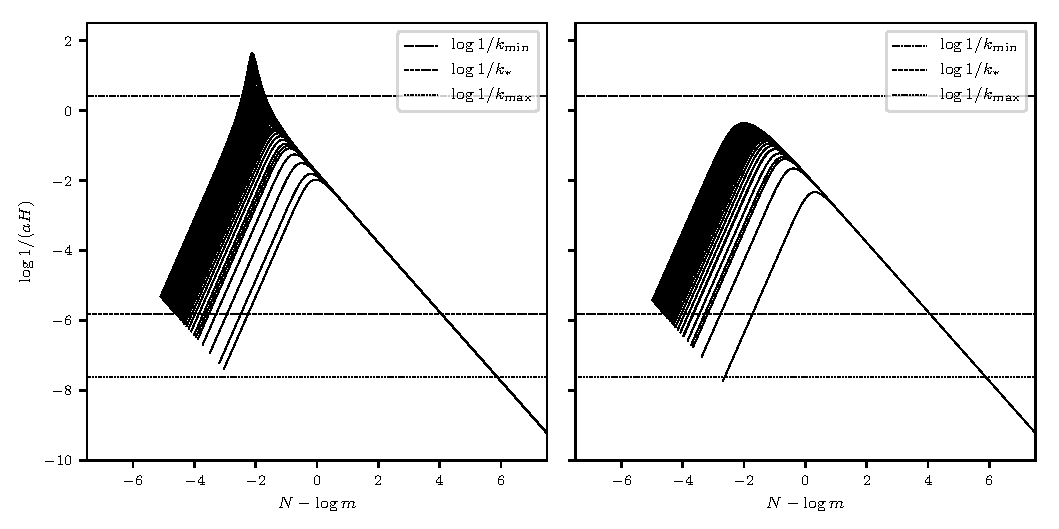
\includegraphics[width=\textwidth]{./figures/horizon_kinetic.pdf}
    \begin{itemize}
        \item Evolution for closed and open cases, such that $N_*=50$.
        \item Inflation preceded by a kinetically dominated phase $\dot{\phi}^2\gg V(\phi)$.
    \end{itemize}
\end{frame}

\begin{frame}
    \frametitle{Primordial vs present-day curvature}
    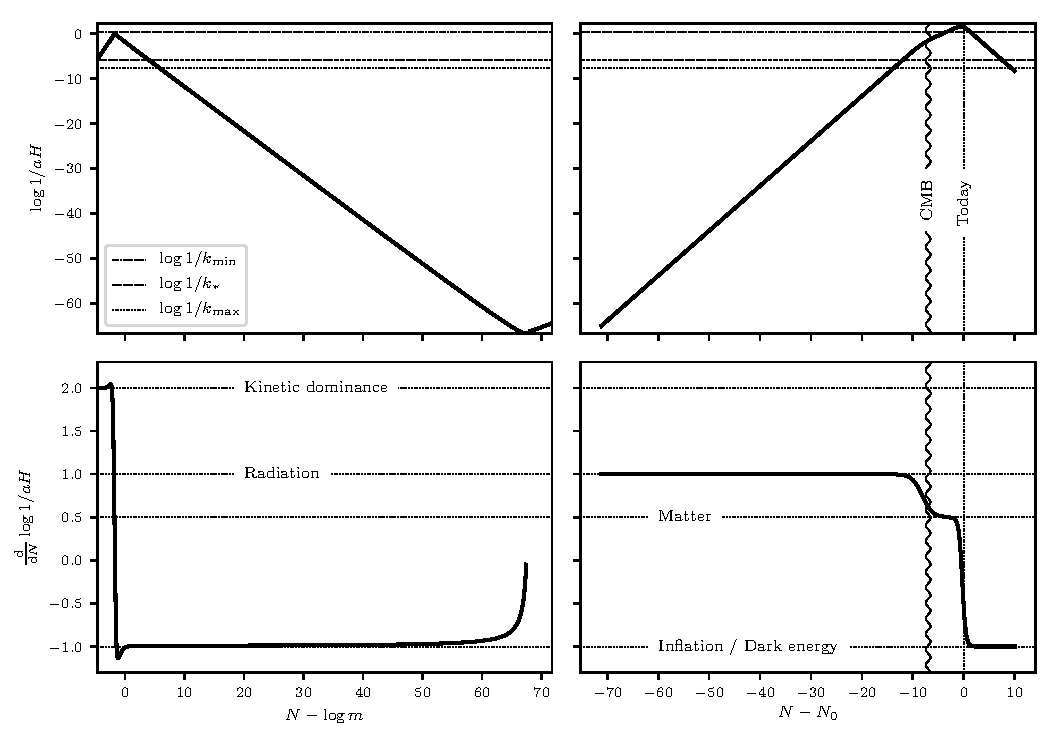
\includegraphics[width=\textwidth]{./figures/horizon_history.pdf}
\end{frame}

\begin{frame}
    \frametitle{Kinetically dominated power spectra}
    \framesubtitle{primordial power spectrum}
    \begin{figright}[0.3]{./figures/pps_Nstar.pdf}
        \begin{itemize}
            \item Eternal inflating models have $\mathcal{P} = A_s {\left(k/k_*\right)}^{n_s-1}$
            \item Finite amount of inflation introduces cutoff and oscillations. 
            \item Hergt et al 2018 (arXiv:1809.07737)
        \end{itemize}
    \end{figright}
\end{frame}

\begin{frame}
    \frametitle{Kinetically dominated power spectra}
    \framesubtitle{CMB power spectrum}
    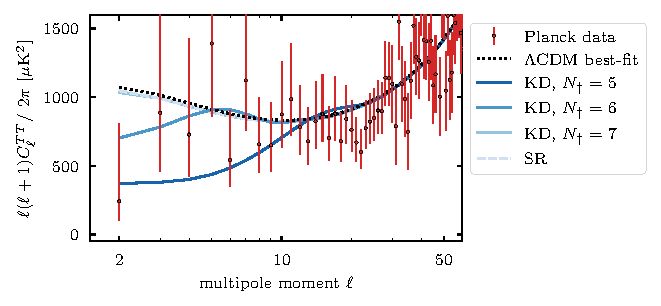
\includegraphics[width=\textwidth]{./figures/cmb_KD_Ndagg.pdf}
    \begin{itemize}
        \item Flat case can reproduce suppression of power
        \item Oscillations have wrong location to explain $\ell \sim 30$ feature.
    \end{itemize}
\end{frame}

\begin{frame}
    \frametitle{Kinetically dominated power spectra}
    \framesubtitle{Parameter estimation and model comparison}
    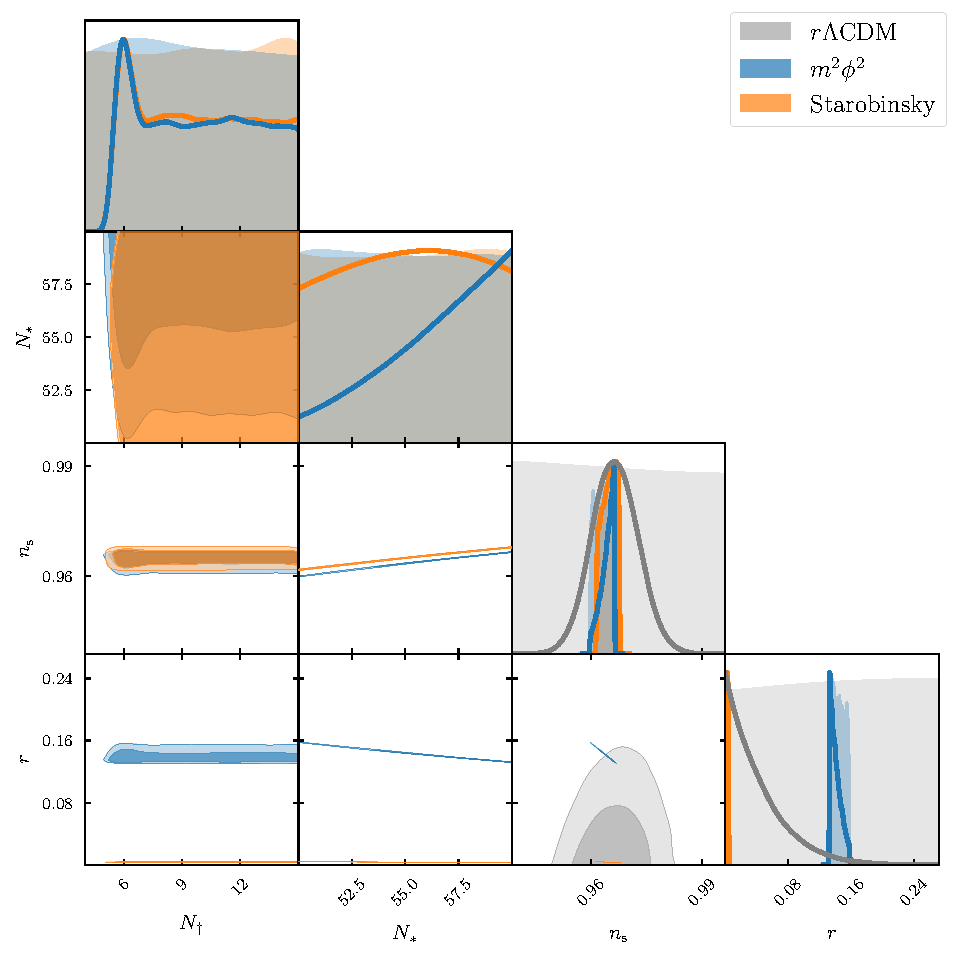
\includegraphics[width=0.6\textwidth]{./figures/cosmo_nrNN.pdf}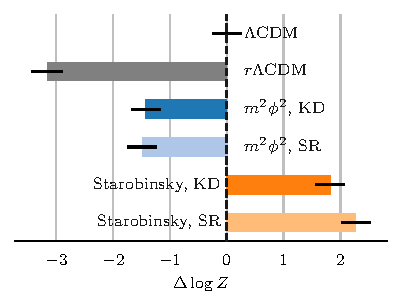
\includegraphics[width=0.4\textwidth]{./figures/cosmo_evidences.pdf}
\end{frame}

\begin{frame}
    \frametitle{Power spectra with primordial curvature.}
    \begin{figright}[0.3]{./figures/dCl.pdf}
    \begin{itemize}
        \item Primordial curvature is able to move oscillation to correct location
        \item Preliminary results: Need full constraint pipeline.
        \item Discretised PPS in closed case.
    \end{itemize}
    \end{figright}
\end{frame}



\begin{frame}
    \frametitle{Computing the primordial power spectrum}
    \begin{itemize}
        \item Comoving curvature perturbation $\Rk$, Power spectrum $\mathcal{P}(k) \propto |\Rk|^2$
        \item Mukhanov-Sasaki equation:
    \end{itemize}
\only<1>{%
\begin{equation*}
    0=
    \dprm{\Rk}
    +2\frac{\prm{z}}{z}\prm{\Rk}
    +\K^2\Rk
\end{equation*}
}
\only<2->{%
\begin{equation*}
    0=
    \dprm{\Rk}
    +\left[2\frac{\prm{z}}{z} +  2K\mathcal{E}\frac{\mathcal{H}  - \frac{\prm{z}}{z} }{\K^2 + K\mathcal{E}}\right]\prm{\Rk}
    +\left[\K^2 + K \frac{\K^2 - K\mathcal{E}- \frac{2\K^2}{\mathcal{H}} \frac{\prm{z}}{z}}{\K^2 + K\mathcal{E}}\right]\Rk
\end{equation*}
}
\onslide<2->{%
    \begin{equation*}
    \mathcal{E} = \mathcal{H}/\dot{\phi}^2
    \end{equation*}
\begin{align*}
    \K^2 &= k(k+2)-3 & K>0 \\
    \K^2 &= k^2 & K=0 \\
    \K^2 &= k^2+3 & K<0
\end{align*}
}

\end{frame}

\begin{frame}
    \frametitle{Problems to be overcome}
    \begin{itemize}
        \item How to set initial condition on $\Rk$ for low-$\K$ modes?
            \begin{itemize}
                \item Usually do so by invoking Bunch-Davies vacuum, which is tied to eternal inflation
                \item Both when and how they are set becomes important
            \end{itemize}
        \item Computing the MS equation numerically becomes bottleneck in computation: Need faster integrators.
        \item Must take care with properly discretised spectra
    \end{itemize}
\end{frame}

\begin{frame}
    \frametitle{Runge-Kutta-Wentzel-Kramers-Brillioun methods}
    \begin{figright}[0.3]{./figures/RKWKB.pdf}
        \begin{itemize}
            \item Rapid solving of equations with oscillatory solutions.
            \item Runge-Kutta based on Taylor series
            \item Replace polynomials with oscillating solutions (e.g.\ Airy, Bessel or WKB).
        \end{itemize}
    \end{figright}
\end{frame}

\begin{frame}
    \frametitle{Further reading}
    \begin{itemize}
        \item Kinetic initial conditions: Handley et al.\ 2015 (arXiv:1401.2253)
        \item Quantum Kinetic Dominance: Handley et al.\ 2016 (arXiv:1607.04148)
        \item Kinetic dominance: Hergt et al.\ 2018 (arXiv:1809.07185)
        \item Kinetic constraints: Hergt et al.\ 2018 (arXiv:1809.07737)
        \item Mukhanov-Sasaki evolution: Haddadin et al..\ 2018 (arXiv:1809.11095)
    \end{itemize}
\end{frame}

\end{document}
